\documentclass[a4paper, 11pt]{article}
\usepackage{fullpage}
\usepackage{mathtools, nccmath}
\usepackage{graphicx}
\usepackage{float}
\renewcommand{\figurename}{Fig.}
\renewcommand{\refname}{Bibliografia}

\begin{document}
%Header
\noindent
\large\textbf{Corso di Metodi di Ottimizzazione} \hfill \textbf{Gruppo E} \\
\normalsize A.A. 2018/2019 \hfill Ing. Saverio Del Prete \\
Prof. Raffaele Martone \hfill Ing. Bernardo Giordano \\
\hphantom{}\hfill Ing. Lucia Migliaccio

\section*{Traccia del problema}

Progetto ottimo di un campo magnetico con incognite geometriche e di corrente di
una spira.

\section*{Descrizione del sistema fisico}

Il sistema è composto da un certo numero di spire
simmetriche (supporremo $n=6$) concentriche rispetto allo
stesso asse $z$. I parametri di
progetto, ovvero posizione, raggio e intensità di corrente, sono noti per tutte
le spire tranne che per una coppia.

\begin{figure}[H]
	\centering
	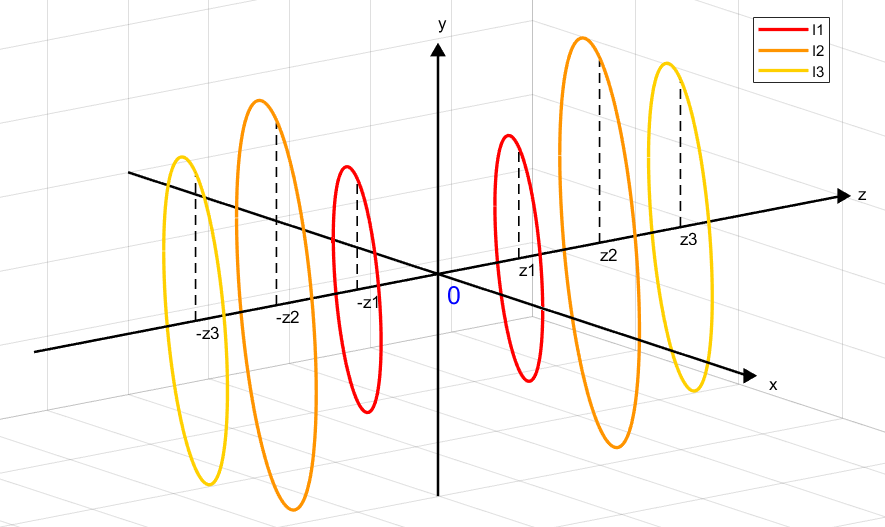
\includegraphics[width=14cm]{assets/figure1}
	\caption{Sistema fisico posizionato nel piano $xyz$.}
\end{figure}

\noindent
Il campo magnetico generato dalla corrente circolante nelle spire può essere
valutato sull’asse utilizzando la legge di Biot-Savart. La legge di Biot-Savart
ci permette di valutare il campo magnetico B prodotto in un punto dello spazio
da una spira percorsa da corrente elettrica. Siccome il sistema è composto da 6
spire, il campo magnetico complessivo si otterrà mediante sovrapposizione degli
effetti di tutte le spire. \\
Il campo magnetico sull’asse di una spira caratterizzata da una corrente $I$,
lunghezza $L$, raggio $R$ e posizione $z$, si valuta come
\[dB_{z}=\frac{\mu_{0}IdL}{4\pi}\frac{R}{\left(z^{2}+R^{2}\right)^{3/2}}\]
L’integrale di $dL$ risulta essere proprio la circonferenza della spira, ovvero
$2{\pi}R$.
Integrando quindi, si ricava la funzione del campo magnetico sull'asse
\[B_{z}=\frac{\mu_{0}}{4\pi}\frac{2{\pi}R^{2}I}{\left(z^{2}+R^{2}\right)^{3/2}}=\frac{\mu_{0}}{2}\frac{R^{2}I}{\left(z^{2}+R^{2}\right)^{3/2}}\]
Siano $Z_{i}$, $R_{i}$ e $I_{i}$ rispettivamente la
posizione, il raggio e la corrente relative alla spira
$i$-esima. \\
Sia inoltre $n=6$ il numero complessivo delle spire facenti
parte del sistema.
Considerando adesso la sovrapposizione degli effetti di tutte le spire del
sistema, e tenendo presente che le spire sono simmetriche rispetto al piano $xy$,
il campo magnetico complessivo sull’asse $z$ varrà

\begin{align*}
	B_{z}
		&=\frac{\mu_{0}}{4{\pi}}\left(\sum_{i=1}^{n/2}\frac{2{\pi}I_{i}R_{i}^{2}}{\left(\left(Z_{i}-z\right)^{2}+R_{i}^{2}\right)^{3/2}}+\frac{2{\pi}I_{i}R_{i}^{2}}{\left(\left(Z_{i}+z\right)^{2}+R_{i}^{2}\right)^{3/2}}\right)\\
		&=\frac{\mu_{0}}{2}\left(\sum_{i=1}^{n/2}\frac{I_{i}R_{i}^{2}}{\left(\left(Z_{i}-z\right)^{2}+R_{i}^{2}\right)^{3/2}}+\frac{I_{i}R_{i}^{2}}{\left(\left(Z_{i}+z\right)^{2}+R_{i}^{2}\right)^{3/2}}\right)
\end{align*}

\begin{thebibliography}{9}
	% \bibitem{id}Author\emph{title}[online]. Editor.
\end{thebibliography}
\end{document}